\documentclass[acmtog,nonacm,screen]{acmart}

\usepackage{tikz}
\usetikzlibrary{positioning,fit,calc,arrows.meta,backgrounds}
\usepackage{xspace}
\usepackage{amsmath}
\usepackage{array}

% palette shared with the figures (reference data-viz palette)
\definecolor{vizblue}{HTML}{2A78D6}
\definecolor{vizorange}{HTML}{EB6834}
\definecolor{vizaqua}{HTML}{1BAF7A}
\definecolor{vizgray}{HTML}{898781}
\definecolor{vizink}{HTML}{0B0B0B}
\definecolor{vizink2}{HTML}{52514E}
\definecolor{vizgrid}{HTML}{E1E0D9}
\definecolor{vizwash}{HTML}{EEF4FC}

\newcommand{\tps}{\,tok/s\xspace}
\newcommand{\us}{\,\textmu{}s\xspace}
\newcommand{\ms}{\,ms\xspace}
\newcommand{\ie}{i.e.,\xspace}
\newcommand{\eg}{e.g.,\xspace}
\newcommand{\ours}{\textsc{FastPath}\xspace}
\setlength{\emergencystretch}{2.5em}
\urlstyle{tt}
\makeatletter\g@addto@macro\UrlBreaks{\do\_\do\=}\makeatother

\setcopyright{none}
\settopmatter{printacmref=false}
\renewcommand\footnotetextcopyrightpermission[1]{}

\begin{document}

\title{One User, One A100: Making a 27B Hybrid-Attention LLM Fast for Agentic Coding}
\subtitle{Split-KV GQA-packed speculative attention, W8A16 decode GEMMs over W8A8 weights, and an agent-aware serving stack}

\author{Tianhao Zang}
\authorsaddresses{}

\begin{abstract}
We report on deploying \emph{Qwen3.8-27B} (W8A8-INT8, 64 layers of which 48 are Gated DeltaNet and 16 are
full attention) on a single NVIDIA A100~80GB as a private, Anthropic-compatible endpoint for one user driving the
Claude Code agent, and on making it as fast as possible \emph{without changing what the model computes}. Profiling
the stock vLLM stack shows that at the context lengths an agent actually works at (tens of thousands of tokens), half
of every decode step is spent in FlashAttention-2 verifying speculative tokens, because its variable-length path
neither splits the KV sequence nor shares KV reads across the six query heads of a GQA group. We replace that path
with a split-KV, GQA-packed kernel that is $13.9\times$ faster at 38K tokens and reads the KV cache at
1.39\,TB/s (83\% of the device's copy bandwidth); we replace the decode-time W8A8 GEMMs by a W8A16 kernel that reads
the very same int8 weights 13--20\% faster with $5\times$ lower numerical error; we draft with an int8 copy of the
LM head and sample drafts probabilistically, which keeps speculative decoding exact while raising acceptance by
7--11\%. Together these make single-stream decoding $1.11$--$1.30\times$ faster on short prompts and $2.13\times$
faster at 38K context. A chat-template change that keeps Claude Code's per-turn system reminders in place lifts
prefix-cache hit rates in a replayed agent loop from 31--34\% to 94--96\% and cuts time-to-first-token per tool step
by $9.5\times$. We release the plugin, the deployment scripts, every benchmark, and the raw measurements behind each
figure.
\end{abstract}

\keywords{LLM inference, speculative decoding, attention kernels, quantization, KV cache, agentic coding}

\begin{teaserfigure}
  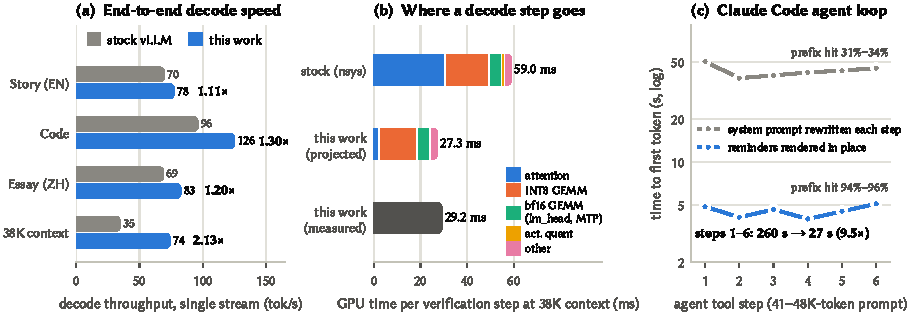
\includegraphics[width=\textwidth]{figures/fig_teaser.pdf}
  \caption{\textbf{Headline results} on one A100 80GB PCIe with the GPU to ourselves. (a)~Single-stream decode
  throughput of stock vLLM~0.31 (MTP speculative decoding, $k{=}2$) versus this work (all three kernel fast paths,
  $k{=}4$). (b)~GPU time per speculative verification step at 38K tokens of context: measured with Nsight Systems
  for the stock stack, projected for ours from per-kernel microbenchmarks, and measured end to end for ours (step time
  $=$ accepted tokens per step\,/\,throughput). (c)~Time to first token in a replayed Claude Code agent loop when the
  agent's per-turn system reminders invalidate the cached prompt (gray) versus when they are rendered in place (blue).}
  \Description{Three panels. Panel a: paired horizontal bars of decode throughput for four workloads; this work is
  1.11, 1.30, 1.20 and 2.13 times faster than stock vLLM. Panel b: stacked bars of per-step GPU time at 38K context,
  59.0 ms for stock (attention dominates), 27.3 ms projected and 29.2 ms measured for this work. Panel c: time to first
  token per agent step on a log axis, about 40 to 50 seconds for the stock template and about 4 to 5 seconds with the
  patched template.}
  \label{fig:teaser}
\end{teaserfigure}

\maketitle

% =====================================================================================================
\section{Introduction}

Agentic coding tools issue a long sequence of requests that share almost all of their prompt: a fixed system
prompt, a few dozen tool schemas, and an ever-growing transcript of tool calls and results. Each request is followed
by a short to medium generation. For a single user the figure of merit is therefore not aggregate throughput but the
latency of one stream at long context: how quickly the next tool call is decided (time to first token, TTFT) and how
fast its arguments and the following prose are written (decode rate).

We serve \emph{Qwen3.8-27B}, a W8A8-INT8 checkpoint of a 27-billion-parameter hybrid model in the
Qwen3~\cite{qwen2025qwen3} line, on one NVIDIA A100 80GB PCIe in a shared server, behind an Anthropic Messages API so
that the Claude Code agent~\cite{anthropic_claude_code} can use it unmodified. The engine is
vLLM~\cite{kwon2023vllm} 0.31 with multi-token-prediction (MTP) speculative
decoding~\cite{gloeckle2024mtp,deepseek2024v3,leviathan2023speculative}, prefix caching and CUDA graphs: a strong,
modern baseline. Our constraint was strict: \emph{no loss of capability}. We did not shrink the context, quantize
further, prune, or replace the sampler. Every change either computes the same function as the code it replaces or
computes it more precisely, and speculative decoding stays distribution-exact.

\paragraph{Contributions.}
\begin{itemize}
\item A profile of where a speculative decode step goes for a hybrid GQA model at agentic context lengths, showing
that the attention verification path, not the weight GEMMs, dominates beyond a few thousand tokens (\S\ref{sec:profile}).
\item A split-KV, GQA-packed attention kernel for uniform speculative-verification batches that is exact,
CUDA-graph safe, and $9$--$16\times$ faster than FlashAttention-2 from 8K to 100K tokens (\S\ref{sec:attention}).
\item A W8A16 decode GEMM that reads the int8 weights in the layout the W8A8 CUTLASS kernel already uses, so prefill
keeps the int8 tensor cores while decode becomes faster and $5\times$ more accurate, at zero memory cost
(\S\ref{sec:linear}).
\item Exact speculative-decoding improvements: an int8 draft LM head and probabilistic drafting (\S\ref{sec:spec}).
\item Agent-aware serving: a prefix-cache-preserving chat template, Anthropic-style authentication, effort mapping
and a self-healing tunnel for the client (\S\ref{sec:agent}, \S\ref{sec:reliability}).
\end{itemize}
All three kernel changes ship as a vLLM plugin of about 500 lines with one environment switch each; the repository contains the
deployment, the benchmarks and the raw numbers behind every figure in this report.

% =====================================================================================================
\section{System Overview}
\label{sec:system}

\begin{figure*}[t]
\centering
\resizebox{0.94\textwidth}{!}{%
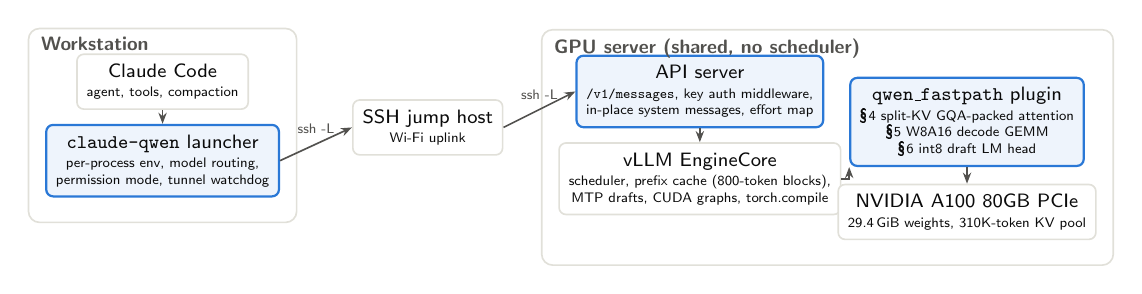
\begin{tikzpicture}[
  font=\sffamily\scriptsize, >={Stealth[length=4pt]},
  box/.style={draw=vizgrid, line width=0.6pt, rounded corners=2.5pt, fill=white, inner sep=3.5pt, align=center, text=vizink},
  ours/.style={box, draw=vizblue, line width=0.8pt, fill=vizwash},
  zone/.style={draw=vizgrid, line width=0.6pt, rounded corners=4pt, inner sep=6pt},
  lab/.style={font=\sffamily\scriptsize\bfseries, text=vizink2, anchor=north west},
  link/.style={->, draw=vizink2, line width=0.6pt},
  note/.style={font=\sffamily\tiny, text=vizink2, align=center}]
% workstation
\node[box] (cc) {Claude Code\\[-1pt]{\tiny agent, tools, compaction}};
\node[ours, below=5pt of cc] (launch) {\texttt{claude-qwen} launcher\\[-1pt]{\tiny per-process env, model routing,}\\[-2pt]{\tiny permission mode, tunnel watchdog}};
\node[zone, fit=(cc)(launch), inner ysep=9pt] (ws) {};
\node[lab] at (ws.north west) {\,Workstation};
% jump
\node[box, right=26pt of launch, yshift=12pt] (jump) {SSH jump host\\[-1pt]{\tiny Wi-Fi uplink}};
% server
\node[ours, right=26pt of jump, yshift=13pt] (api) {API server\\[-1pt]{\tiny \texttt{/v1/messages}, key auth middleware,}\\[-2pt]{\tiny in-place system messages, effort map}};
\node[box, below=5pt of api] (engine) {vLLM EngineCore\\[-1pt]{\tiny scheduler, prefix cache (800-token blocks),}\\[-2pt]{\tiny MTP drafts, CUDA graphs, torch.compile}};
\node[ours, right=9pt of api, yshift=-11pt] (plug) {\texttt{qwen\_fastpath} plugin\\[-1pt]{\tiny \S4 split-KV GQA-packed attention}\\[-2pt]{\tiny \S5 W8A16 decode GEMM}\\[-2pt]{\tiny \S6 int8 draft LM head}};
\node[box, below=6pt of plug] (gpu) {NVIDIA A100 80GB PCIe\\[-1pt]{\tiny 29.4\,GiB weights, 310K-token KV pool}};
\node[zone, fit=(api)(engine)(plug)(gpu), inner ysep=9pt] (srv) {};
\node[lab] at (srv.north west) {\,GPU server (shared, no scheduler)};
% links
\draw[link] (cc) -- (launch);
\draw[link] (launch.east) -- node[note, above] {ssh -L} (jump.west);
\draw[link] (jump.east) -- node[note, above] {ssh -L} (api.west);
\draw[link] (api) -- (engine);
\draw[link] (engine.east) -| (plug.south west);
\draw[link] (plug) -- (gpu);
\end{tikzpicture}}
\caption{\textbf{Deployment.} Blue outlines mark components we wrote or changed; everything else is stock. The client
reaches the loopback-only API through two SSH hops; the plugin is loaded by vLLM's general-plugin entry point in every
engine process.}
\Description{Block diagram. On a workstation, Claude Code talks to the claude-qwen launcher. The launcher opens an
SSH tunnel through a jump host to the API server on the GPU server. The API server feeds the vLLM engine core, which
uses the qwen fastpath plugin running on the A100 GPU.}
\label{fig:arch}
\end{figure*}

Figure~\ref{fig:arch} shows the deployment and Table~\ref{tab:model} the model and hardware. The model interleaves
three Gated DeltaNet~\cite{yang2025gateddeltanet} linear-attention layers with one full-attention layer; the full
attention uses grouped-query attention~\cite{ainslie2023gqa} with $G{=}6$ query heads per KV head and a head
dimension of 256, so one cached token costs 4\,KiB per full-attention layer and 64\,KiB in total. Linear layers are
stored as per-output-channel int8 weights, and activations are quantized per token at run time (W8A8,
\cite{dettmers2022llmint8,xiao2023smoothquant}). A single MTP layer predicts further tokens from the last hidden
state; vLLM uses it as the drafter for speculative decoding.

\paragraph{Serving configuration.} vLLM~0.31.0 (V1 engine) serves a 131{,}072-token context with
\texttt{gpu-memory-utilization} 0.72, which leaves room for a co-tenant's jobs and gives a 310K-token KV pool; prefix
caching is on (the hybrid layers are cached in vLLM's ``align'' mode, see \S\ref{sec:agent}); CUDA graphs are captured
for every batch size up to 32 and in coarser steps beyond (\texttt{--performance-mode interactivity}); and speculative decoding uses the MTP head
with $k$ draft tokens. The Anthropic endpoint is vLLM's own; we add an ASGI middleware that accepts
\texttt{x-api-key} or bearer tokens with a constant-time comparison and guards every route but \texttt{/health}
(vLLM's built-in key check accepts only bearer tokens and guards only a few route prefixes).

\begin{table}[t]
\caption{Model and hardware.}
\label{tab:model}
\small
\begin{tabular}{@{}l>{\raggedright\arraybackslash}p{0.63\columnwidth}@{}}
\toprule
Layers & 64: 48 Gated DeltaNet + 16 full attention \\
Hidden / MLP width & 5{,}120 / 17{,}408 \\
Attention & 24 query heads, 4 KV heads ($G{=}6$), $d{=}256$ \\
Vocabulary & 248{,}320 (untied bf16 LM head, 2.54\,GB) \\
Quantization & W8A8 int8: per-channel weights, per-token activations \\
Weights in memory & 29.4\,GiB (int8 body 24.3\,GB) \\
Draft model & 1 MTP layer (shares the LM head) \\
Context & 262{,}144 native, 131{,}072 served \\
\midrule
GPU & NVIDIA A100 80GB PCIe, 108 SMs, 1410\,MHz \\
Measured bandwidth & 1{,}671\,GB/s copy; 1{,}702\,GB/s bf16 GEMV \\
Software & vLLM 0.31.0, PyTorch 2.13, CUDA 13.0 \\
\bottomrule
\end{tabular}
\end{table}

\paragraph{Methodology.} Unless noted, throughput is single-stream decode of a 1{,}024-token completion (600 tokens for
the 38K-context prompt) with thinking disabled and the model's default sampling (temperature 1.0, top-$p$ 0.95,
top-$k$ 20), averaged over two runs, with the GPU otherwise idle. Three prompts probe different acceptance regimes:
an English story (low acceptance), Python code (high) and a Chinese essay. ``38K context'' decodes after a
37{,}932-token prompt. Kernels are timed by replaying 20--30 calls captured in a CUDA graph and taking the best of
five replays. The server is shared and has no scheduler; \S\ref{sec:contention} quantifies what co-tenants cost.

% =====================================================================================================
\section{Where a Decode Step Goes}
\label{sec:profile}

A speculative step runs the target model once over $1{+}k$ positions (the last accepted token plus $k$ drafts), then
the drafter $k$ times. Because the batch is tiny, the target pass is memory-bound: it must stream the 24.3\,GB of
int8 body weights and the 2.54\,GB bf16 LM head, a floor of 16\,ms per step at the measured 1.67\,TB/s
\cite{williams2009roofline}. At short context the stock stack takes 28.5\ms per step including drafting.

At 38K tokens the picture changes. Figure~\ref{fig:teaser}b breaks down 26 verification steps traced with Nsight
Systems~\cite{nvidia_nsys} at CUDA-graph-node granularity: FlashAttention-2~\cite{dao2024flashattention2} takes
30.5\ms per step (52\%), more than all int8 GEMMs together (18.9\ms, 32\%); bf16 GEMMs for the target and draft LM
heads take 5.6\ms, activation quantization 0.9\ms and everything else 3.1\ms. Each of the 16 full-attention layers
spends 1.75\ms on attention, while reading that layer's 38K-token KV cache once (156\,MB) would take 0.09\ms at peak
bandwidth.

\paragraph{Why FlashAttention-2 is slow here.} Verification gives every request $Q{=}1{+}k$ query tokens, so vLLM takes
FlashAttention-2's variable-length path. That path does not split the KV sequence (requesting more than one split is
rejected by vLLM's wrapper and by the kernel), so the grid has one block per query head: 24 blocks on a 108-SM GPU,
each streaming its KV head from HBM. With $G{=}6$, each KV head is read six times, and each block fills only $Q$ of its
64 tile rows. FlashAttention-2 does pack a GQA group into one tile through its ``head swap'' trick, and
Flash-Decoding~\cite{dao2023flashdecoding} splits the sequence, but both only when the query length is one, \ie for
non-speculative decoding. Speculative decoding falls between the cases. Neither of vLLM's other backends helps:
Triton attention is slower still, and FlashInfer~\cite{ye2025flashinfer} supports only piecewise CUDA graphs with
speculative decoding, which costs more at short context than it saves at long context
(Figure~\ref{fig:attention}c).

% =====================================================================================================
\section{Split-KV GQA-Packed Verification Attention}
\label{sec:attention}

\begin{figure*}[t]
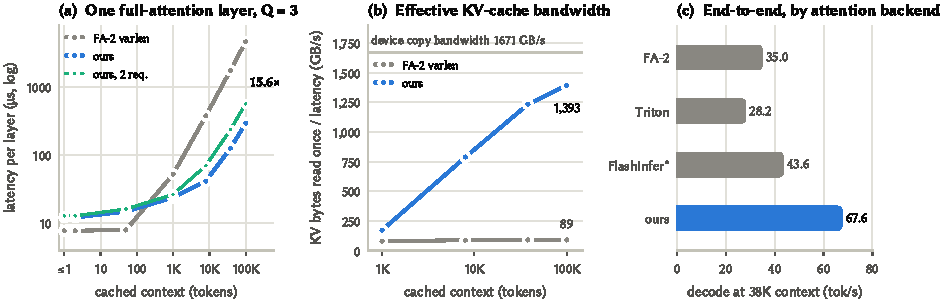
\includegraphics[width=\textwidth]{figures/fig_attention.pdf}
\caption{\textbf{Verification attention.} (a)~Latency of one full-attention layer with $Q{=}3$ query tokens (one
request, and two requests of slightly different lengths) over a paged KV cache. (b)~Effective bandwidth: the bytes of
KV a layer must read once, divided by its latency. FlashAttention-2 plateaus near 90\,GB/s because it reads every KV
head six times from only 24 thread blocks; ours approaches the device copy bandwidth. (c)~End-to-end decode rate at
38K context with each attention implementation (other kernels stock, $k{=}2$). *FlashInfer runs with piecewise CUDA
graphs only, and its two runs differed by 28\%.}
\Description{Three panels. Panel a: log-log latency versus cached context; FlashAttention-2 rises to 4.6 ms at 100K
tokens while ours stays at 0.29 ms, 15.6 times lower. Panel b: effective bandwidth; ours rises to 1393 GB/s at 100K
tokens, close to the 1671 GB/s copy bandwidth, while FlashAttention-2 stays near 89 GB/s. Panel c: decode at 38K
context is 35.0, 28.2, 43.6 and 67.6 tokens per second for FlashAttention-2, Triton, FlashInfer and ours.}
\label{fig:attention}
\end{figure*}

We handle the uniform batches that speculative verification produces (every request has the same $1 < Q \le 8$)
with two Triton~\cite{tillet2019triton} kernels and leave everything else (prefill, mixed batches, $Q{=}1$) on
FlashAttention-2.

\paragraph{Decomposition.} Let request $b$ have $L_b$ cached tokens including this step's $Q$, so its prefix is
$P_b{=}L_b{-}Q$. Query $i$ ($0 \le i < Q$) attends causally to positions $\le P_b + i$. Split the keys into the prefix
$[0, P_b)$, which every query sees in full, and the $Q$ in-flight tokens, which it sees causally. Softmax attention
over a union of disjoint key sets is recovered exactly from per-set partial results by their log-sum-exp
(LSE)~\cite{milakov2018online,dao2023flashdecoding}: if part $j$ yields the normalized output $o_j$ and
$\ell_j = \log\sum \exp(s)$ over its scores, then
\begin{equation}
o \;=\; \sum_j \frac{e^{\ell_j - m}}{\sum_{j'} e^{\ell_{j'} - m}}\; o_j, \qquad m = \max_j \ell_j .
\end{equation}

\paragraph{Prefix kernel.} Because the prefix is non-causal for all $Q$ queries, the $R{=}QG$ query rows that share a
KV head (18 rows for $Q{=}3$) are packed into a single tile: the KV head is read once for all of them, and the
$16 \times 32$ tensor-core MMA tiles are mostly full. The prefix is split into $S$ chunks of at least 128 tokens, and
the grid has $S \times B \times H_{kv}$ blocks; each block walks its chunk through the block table (800-token pages),
keeps an online softmax in base 2 and writes a partial output and LSE. With $S{=}64$ and $H_{kv}{=}4$ a single
request fills 256 blocks.

\paragraph{Suffix-and-combine kernel.} One program per (token, head) row attends to the $\le Q$ in-flight tokens of
its request (read from the same paged cache, as FlashAttention-2 does, so the layer contract is unchanged), then folds
in the active prefix splits with the LSE rule above and writes the final output. It recomputes the split arithmetic
from the sequence length, so the prefix kernel can exit early for empty splits and nothing depends on host-side
values: both grids are fixed for a given batch shape and the pair is captured into vLLM's full CUDA graphs. (We first
tried FlashAttention-2's own \path{fwd_kvcache} entry, which does split and reaches 0.19\ms at 38K with GQA packing,
but it reads the maximum sequence length on the host and invalidates graph capture.)

\paragraph{Correctness and tuning.} Against an fp32 reference over shuffled pages, relative error is
$2.1$--$2.2\times10^{-3}$ versus $2.2$--$2.3\times10^{-3}$ for FlashAttention-2, including the edge cases of an empty
prefix, a request shorter than $Q$, and batched requests of different lengths. A sweep over 216 configurations at each of
1K, 38K and 100K tokens chose one setting, within 3\% of the best per-length configuration at 38K and 100K:
$S{=}64$, a minimum chunk of 128, $32$-token KV tiles, 4 warps and 2 stages.

\paragraph{Results.} Figure~\ref{fig:attention}a,b and Table~\ref{tab:attention}: from 1K to 100K tokens, attention
is $2.2$--$15.6\times$ faster and reaches 1.39\,TB/s, 83\% of the copy bandwidth. Below about 100 tokens the second
launch makes ours 5--7\us slower per layer, under 0.1\ms per step. End to end at 38K tokens, decoding goes from 35.0 to
67.6\tps with no other change.

\begin{table}[t]
\caption{Latency of one full-attention layer (\textmu{}s), $Q$ query tokens per request over a paged KV cache.}
\label{tab:attention}
\small
\setlength{\tabcolsep}{4.2pt}
\begin{tabular}{@{}rrrrrrr@{}}
\toprule
 & \multicolumn{2}{c}{$Q{=}3$, 1 req.} & \multicolumn{2}{c}{$Q{=}4$, 1 req.} & \multicolumn{2}{c}{$Q{=}3$, 2 req.} \\
\cmidrule(lr){2-3}\cmidrule(lr){4-5}\cmidrule(l){6-7}
Context & FA-2 & ours & FA-2 & ours & FA-2 & ours \\
\midrule
0      & 7.8    & 7.2   & 8.3    & 7.0   & 7.8    & 8.7 \\
50     & 8.0    & 14.9  & 8.0    & 15.3  & 8.1    & 16.2 \\
1K     & 52.5   & 23.9  & 52.5   & 24.4  & 52.7   & 26.5 \\
8K     & 376.4  & 41.6  & 376.6  & 43.8  & 376.2  & 70.2 \\
38K    & 1750.8 & 126.2 & 1753.3 & 129.1 & 1749.6 & 236.1 \\
100K   & 4589.5 & 294.1 & 4588.7 & 294.7 & 4600.8 & 565.5 \\
\bottomrule
\end{tabular}
\end{table}

% =====================================================================================================
\section{W8A16 Decode GEMMs over W8A8 Weights}
\label{sec:linear}

\begin{figure*}[t]
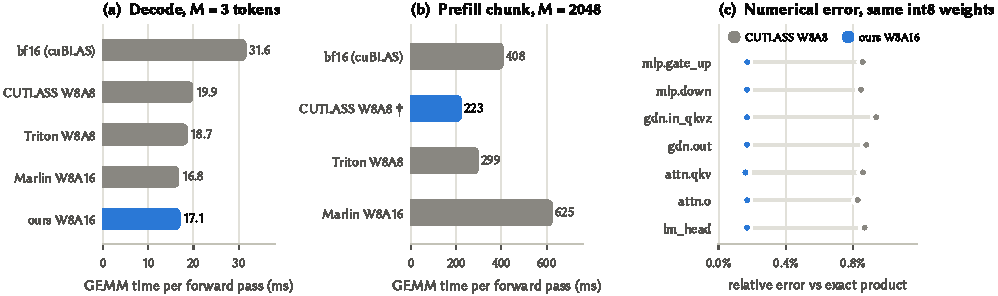
\includegraphics[width=\textwidth]{figures/fig_linear.pdf}
\caption{\textbf{Linear layers.} (a)~Time of all int8 GEMMs in one forward pass at decode batch size ($M{=}3$
tokens), per implementation. (b)~The same for a 2048-token prefill chunk; $\dagger$ ours keeps CUTLASS W8A8 for $M>16$.
(c)~Relative error against the exact product for the same int8 weights: rounding activations to int8 costs about
0.9\%, keeping them in bf16 costs 0.17\%.}
\Description{Three panels. Panel a: GEMM time per decode forward pass: bf16 31.6 ms, CUTLASS W8A8 19.9 ms, Triton W8A8
18.7 ms, Marlin W8A16 16.8 ms, ours 17.0 ms. Panel b: prefill chunk: bf16 408 ms, CUTLASS 223 ms, Triton 299 ms,
Marlin 625 ms. Panel c: relative error per layer type: about 0.86 to 0.94 percent for W8A8 and about 0.17 percent for
our W8A16.}
\label{fig:linear}
\end{figure*}

At decode batch sizes an int8 GEMM moves one byte per weight and does almost no arithmetic per byte, so its speed is
the rate at which it streams weights. vLLM's CUTLASS~\cite{nvidia_cutlass} W8A8 kernel (16$\times$64$\times$128 tiles,
stream-K) reaches 1.15--1.29\,TB/s on this model's shapes and needs a separate per-token activation-quantization
kernel before every GEMM (0.9\ms per step).

\paragraph{Kernel.} Our Triton kernel reads the weight tensor exactly as vLLM stores it for CUTLASS, a $[K, N]$
column-major view of the checkpoint's $[N, K]$ int8 matrix, so no second copy and no repacking are needed. Each block
owns a 32- or 64-column slab and walks $K$ in 128- or 256-element steps, converting int8 to bf16 in registers (exact:
$|w| \le 127$ fits bf16's 8-bit significand) and accumulating $x\,W$ in fp32 on tensor cores with $M$ padded to 16; the
per-channel scale is applied in the epilogue. Narrow-$N$ shapes split $K$ across 2--4 blocks and reduce with fp32
atomics. Tile sizes were tuned per shape at $M{=}3$ (Table~\ref{tab:w8a16cfg}). A dispatcher registered as an opaque
custom op (so \texttt{torch.compile} keeps it as one node) routes $M \le 16$ to this kernel and everything larger to
CUTLASS.

\paragraph{Speed.} The kernel streams weights at 1.31--1.62\,TB/s; over one forward pass the int8 GEMMs take 17.1\ms
instead of 19.7\ms in the same run ($-13\%$), and the activation-quantization kernels disappear
(Figure~\ref{fig:linear}a). Marlin~\cite{frantar2025marlin}, tested in its W8A16 mode, is as fast at decode (16.8\ms)
but needs its own repacked weight layout and is $2.8\times$ slower than CUTLASS on prefill chunks
(Figure~\ref{fig:linear}b). Using it for decode only would mean keeping a second 24.3\,GB copy of the weights, which
would leave almost no memory for the KV cache.

\paragraph{Accuracy.} The product is now exact up to fp32 accumulation and the final bf16 rounding. Against the exact
product the relative error drops from 0.83--0.94\% (W8A8) to 0.16--0.17\% for every layer shape
(Figure~\ref{fig:linear}c). Decode becomes \emph{more} faithful to the checkpoint's weights than the stock kernel,
while prefill is unchanged.

\begin{table}[t]
\caption{Per-shape W8A16 configuration (block $N$, block $K$, split-$K$, warps, stages) and latency at $M{=}3$.}
\label{tab:w8a16cfg}
\small
\setlength{\tabcolsep}{3.6pt}
\begin{tabular}{@{}lrrcrrr@{}}
\toprule
Layer & $N$ & $K$ & config & CUTLASS & ours & TB/s \\
\midrule
mlp.gate\_up  & 34{,}816  & 5{,}120  & 32/256/1/4/3 & 138.3 & 119.7 & 1.49 \\
mlp.down      & 5{,}120   & 17{,}408 & 32/256/2/4/3 & 73.6  & 64.4  & 1.38 \\
gdn.in\_qkvz  & 16{,}384  & 5{,}120  & 32/128/1/4/4 & 69.7  & 59.5  & 1.41 \\
gdn/attn.out  & 5{,}120   & 6{,}144  & 64/128/4/4/3 & 27.1  & 24.0  & 1.31 \\
attn.qkv      & 14{,}336  & 5{,}120  & 32/128/4/4/4 & 64.2  & 54.9  & 1.34 \\
lm\_head (int8) & 248{,}320 & 5{,}120 & 64/256/1/8/3 & 937.4 & 782.6 & 1.62 \\
\bottomrule
\end{tabular}
\end{table}

% =====================================================================================================
\section{Exact Speculative Decoding, Tuned for One Stream}
\label{sec:spec}

\begin{figure}[t]
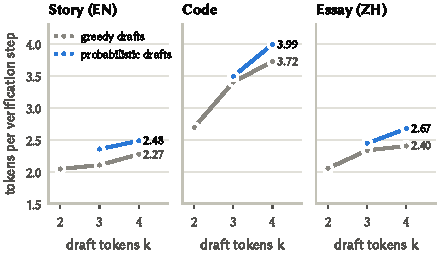
\includegraphics[width=\columnwidth]{figures/fig_spec_accept.pdf}
\caption{\textbf{Acceptance.} Tokens produced per verification step (accepted drafts $+1$) versus the number of draft
tokens. Sampling the drafts from the MTP head's distribution instead of taking its argmax raises acceptance at
temperature 1.0 by 7--11\% at $k{=}4$, and the rejection test keeps the output distribution exact.}
\Description{Three small line charts, one per workload, of tokens per verification step versus k from 2 to 4.
Probabilistic drafts are above greedy drafts: 2.48 versus 2.27 for story, 3.99 versus 3.72 for code, 2.67 versus 2.40
for the Chinese essay at k equals 4.}
\label{fig:accept}
\end{figure}

\begin{figure*}[t]
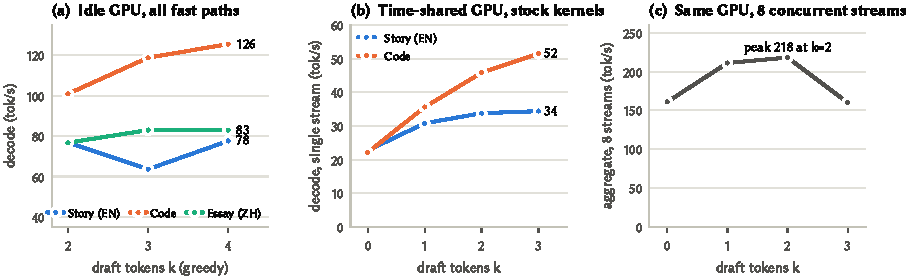
\includegraphics[width=\textwidth]{figures/fig_k_sweep.pdf}
\caption{\textbf{Choosing $k$.} (a)~With the GPU to ourselves and all fast paths, a single stream keeps improving up
to $k{=}4$ (the $k{=}3$ story point is a low outlier; the same configuration with the bf16 draft head gave 73.0\tps).
(b,c)~In our first deployment, on a GPU time-shared with a training job and with stock kernels: drafts help a single
stream at every $k$, while the aggregate rate of eight concurrent streams peaks at $k{=}2$. The best $k$ for one user is
larger than the best $k$ for a serving fleet.}
\Description{Three line charts. Panel a: decode rate versus k for three workloads on an idle GPU, code reaching 126
tokens per second at k equals 4. Panel b: single-stream decode on a shared GPU rising with k for story and code. Panel
c: aggregate throughput of eight streams, 161, 211, 218 and 160 tokens per second for k from 0 to 3.}
\label{fig:ksweep}
\end{figure*}

Speculative decoding~\cite{leviathan2023speculative,chen2023speculative} is exact: drafts are accepted or resampled so
that outputs follow the target distribution. Its benefit depends on the drafter's cost and acceptance rate, so both can
be improved without touching the model's behavior.

\paragraph{Int8 draft LM head.} Every draft token runs the MTP layer and then a 2.54\,GB bf16 LM-head GEMV. We give the
drafter its own int8 copy of the head (per-row scales, 1.27\,GB) and run it through the W8A16 kernel. Only the
proposals change; verification still uses the target's bf16 head, so the outputs are exactly distributed as before. At
$k{=}4$ this raises decode rates by 6--15\% (story 73.5$\to$77.6, code 115.8$\to$125.5, essay 72.3$\to$82.9\tps).
(vLLM 0.31's drafter calls \path{compute_logits} rather than the \path{get_top_tokens} hook its MTP model
exposes, so the patch must replace the former.)

\paragraph{Probabilistic drafts.} vLLM's MTP drafter takes the argmax by default; with
\path{draft_sample_method=probabilistic} it samples from the draft distribution and uses its probabilities in the
acceptance test. At the model's default temperature of 1.0 this is the better proposal: acceptance rises by 9\%, 7\% and
11\% on the three workloads at $k{=}4$ (Figure~\ref{fig:accept}). The production configuration uses it.

\paragraph{How many drafts.} Larger $k$ costs more verification work per step, which a busy server pays across all
streams. Our first deployment, on stock kernels and a time-shared GPU, showed exactly this trade-off
(Figure~\ref{fig:ksweep}b,c): the aggregate of eight streams peaked at $k{=}2$, while a single stream gained up to $k{=}3$.
For one user, after the attention and GEMM fixes made each step cheaper, $k{=}4$ is best (Figure~\ref{fig:ksweep}a);
it reduces the KV pool by 12\% (352K to 310K tokens), which still holds 2.36 full 131K-token contexts.

% =====================================================================================================
\section{Serving an Agent: Keeping the Prefix Cached}
\label{sec:agent}

\begin{figure}[t]
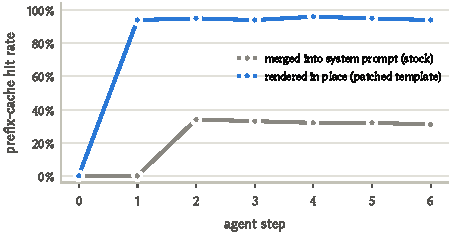
\includegraphics[width=\columnwidth]{figures/fig_prefix.pdf}
\caption{\textbf{Prefix reuse in an agent loop.} Fraction of prompt tokens served from the prefix cache at each step
of a replayed Claude Code session (41K tokens at step 0, growing by 1.1K per step). Stock vLLM merges the agent's
per-turn system reminders into the system prompt, so only the tool definitions that precede it are reused.}
\Description{Line chart of prefix cache hit rate per agent step. The stock template stays at 0 percent for the first
two steps and then 31 to 34 percent; the patched template reaches 94 to 96 percent from step 1 on.}
\label{fig:prefix}
\end{figure}

We captured Claude Code's requests with a logging proxy. Each request carries two cacheable system blocks, about 20
tool schemas, the transcript, and \emph{inline system messages}: an 8K-character environment block after the first user
turn and a short reminder after every later turn. With extended thinking, it also sends an \texttt{effort} level of
\texttt{low}\ldots\texttt{max}.

\paragraph{In-place system messages.} The model's chat template raises an error on any system message that is not
first. vLLM detects this and merges every inline system message into the leading system prompt, which means each new
reminder rewrites text near the start of the prompt and invalidates the cache for everything after it. Because the
template renders tool schemas before the system text, only the tools remain reusable. We changed the template to render
non-leading system messages in place as their own system turns. Replaying a 41K-token session for six tool steps
(Figure~\ref{fig:prefix}, Figure~\ref{fig:teaser}c), the hit rate goes from 31--34\% to 94--96\% and the summed
time-to-first-token from 260\,s to 27\,s. In place is also closer to how the agent intends the reminders to be read.

\paragraph{Per-request headers and hybrid-cache granularity.} Claude Code also prepends a billing header whose hash
changes with every request; dropping it on the client (\path{CLAUDE_CODE_ATTRIBUTION_HEADER=0}) took a 4-turn
session from 0\% to 68\% cache hits before the template fix. The Gated DeltaNet layers have recurrent state that can be
cached only at block boundaries (vLLM ``align'' mode with 800-token blocks here), so up to one block is always
recomputed: a shared 19{,}270-token prompt is served in 1.9\,s instead of 20.0\,s with 93\% of its tokens from cache.

\paragraph{Effort, compaction and permissions.} The template knows three reasoning efforts; we map \texttt{xhigh} and
\texttt{max} to its highest, \texttt{low} to its lowest and everything else to medium. On the client the launcher
declares the true 131K window and starts compaction at 75\% of it. Without that, Claude Code assumes a window
that, together with its 32K output budget, runs into the server's hard limit. The launcher sets all of these per
process and leaves the user's normal \texttt{claude} untouched.

% =====================================================================================================
\section{Results}
\label{sec:results}

\begin{figure}[t]
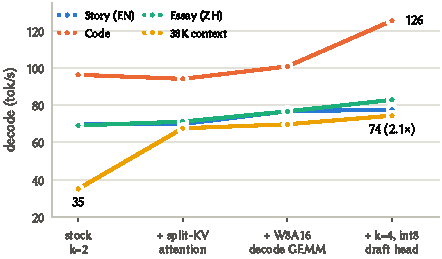
\includegraphics[width=\columnwidth]{figures/fig_ablation.pdf}
\caption{\textbf{Ablation.} Decode rate as the fast paths are added. The attention kernel accounts for the long-context
gain; the GEMM kernel and the speculative-decoding changes for the short-context gains.}
\Description{Line chart with four workloads across four cumulative configurations. The 38K-context curve rises from
35 to 74 tokens per second, mostly at the attention step; code rises from 96 to 126.}
\label{fig:ablation}
\end{figure}

\begin{table*}[t]
\caption{All measured configurations (GPU idle except the last two rows). Decode in \tps; tokens per verification step
in parentheses; ``38K'' is the mean of two decodes after a 37{,}932-token prompt.}
\label{tab:configs}
\small
\begin{tabular}{@{}llrrrrr@{}}
\toprule
Configuration & Drafts & Story (EN) & Code & Essay (ZH) & 38K & KV pool \\
\midrule
Stock vLLM 0.31 (FA-2, CUTLASS W8A8)        & $k{=}2$ greedy & 69.8 (2.00) & 96.4 (2.76)  & 69.1 (1.98) & 35.0 & 352K \\
\quad attention backend: Triton               & $k{=}2$ greedy & 69.6 (2.00) & 93.9 (2.70)  & 70.7 (2.03) & 28.2 & 352K \\
\quad attention backend: FlashInfer           & $k{=}2$ greedy & 48.1 (2.00) & 61.5 (2.68)  & 49.8 (2.00) & 43.6 & 349K \\
+ split-KV GQA-packed attention               & $k{=}2$ greedy & 69.9 (1.99) & 94.2 (2.68)  & 71.2 (2.03) & 67.6 & 346K \\
+ W8A16 decode GEMM                           & $k{=}2$ greedy & 76.8 (2.04) & 100.9 (2.69) & 76.7 (2.05) & 69.8 & 346K \\
\quad $k{=}3$, bf16 draft head                & $k{=}3$ greedy & 73.0 (2.12) & 115.4 (3.36) & 77.1 (2.25) & 71.9 & 320K \\
\quad $k{=}4$, bf16 draft head                & $k{=}4$ greedy & 73.5 (2.32) & 115.8 (3.67) & 72.3 (2.30) & 67.0 & 310K \\
+ int8 draft head                             & $k{=}3$ greedy & 63.6 (2.10) & 118.8 (3.40) & 83.0 (2.33) & 76.4 & 320K \\
+ int8 draft head                             & $k{=}4$ greedy & \textbf{77.6} (2.27) & \textbf{125.5} (3.72) & \textbf{82.9} (2.40) & \textbf{74.4} & 325K \\
\midrule
Production, 6 co-tenant processes             & $k{=}3$ prob.  & 12.2 (2.35) & 18.3 (3.49) & 12.6 (2.44) & 11.6 & 226K \\
Production, 6 co-tenant processes             & $k{=}4$ prob.  & 11.4 (2.48) & 18.4 (3.99) & 12.2 (2.67) & 10.5 & 310K \\
\bottomrule
\end{tabular}
\end{table*}

Table~\ref{tab:configs} lists every configuration we measured, and Figure~\ref{fig:ablation} shows the cumulative
effect. On short prompts the stack is $1.11$--$1.30\times$ faster (story 77.6, code 125.5, essay 82.9\tps), and at 38K
context it is $2.13\times$ faster (74.4\tps), where the stock stack ran at half its story-prompt speed and ours runs within 4--10\%
of its story and essay speeds. The measured step time at 38K, 29.2\ms, is within 7\% of the 27.3\ms projected from the kernel
microbenchmarks (Figure~\ref{fig:teaser}b). Prefill is unchanged by design (it keeps the CUTLASS path): 4.3--5.6K
prompt tokens/s from 2K to 38K tokens before and after. The production configuration adds probabilistic drafting,
whose acceptance gain (Figure~\ref{fig:accept}) we measured only while the GPU was shared. Its idle-GPU throughput is
therefore not reported here.

\paragraph{Capability checks.} The patched server passes the same API test matrix as the stock one: eight
authentication cases, Messages and token counting, extended thinking, tool use, vision, and all five effort levels.
A needle hidden at 30\% and 85\% depth of a 28K-token prompt and at 50\% of a 76K-token prompt is retrieved verbatim
at temperature 0. Claude Code completes a two-turn task through the endpoint (write a statistics module and its tests,
then extend both), and the 22 tests it wrote pass when we rerun them.

\subsection{The cost of sharing a GPU}
\label{sec:contention}

\begin{figure}[t]
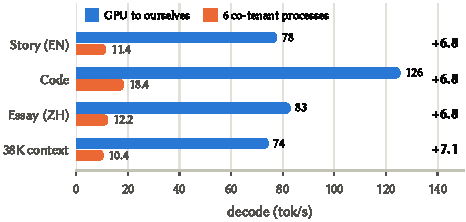
\includegraphics[width=\columnwidth]{figures/fig_contention.pdf}
\caption{\textbf{Co-tenancy.} Decode with the GPU to ourselves versus with six other processes from a co-tenant's
training jobs time-slicing it (no MPS, no scheduler). Idle numbers use greedy $k{=}4$ and contended numbers
probabilistic $k{=}4$, which accepts more, so the slowdown is if anything understated.}
\Description{Paired horizontal bars. Every workload drops by a factor of 6.8 to 7.1, for example code from 126 to 18.4
tokens per second.}
\label{fig:contention}
\end{figure}

The server has no GPU scheduler. When six processes from another user's jobs started on our GPU, each holding only
2\,GB but issuing kernels continuously, every decode rate fell by $6.8$--$7.1\times$ and the 38K-token prefill took
41.3\,s instead of 8.3\,s (Figure~\ref{fig:contention}). Time-slicing between CUDA contexts, not memory, is the
bottleneck, and no kernel optimization in this report changes that. The GPU's MPS daemon with client priorities is
available on this machine and would let the interactive server preempt batch work, but it requires restarting the
co-tenant's jobs under MPS.

% =====================================================================================================
\section{A Self-Healing Client Path}
\label{sec:reliability}

\begin{figure}[t]
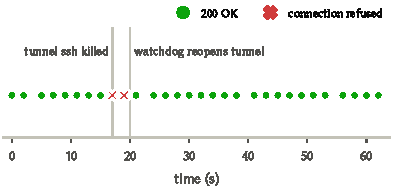
\includegraphics[width=\columnwidth]{figures/fig_tunnel.pdf}
\caption{\textbf{Tunnel recovery.} A client issuing one request every 2.2\,s while the tunnel's SSH process is
killed. The watchdog notices within its 5\,s check period and reopens the tunnel through the next jump-host port; two
requests fail.}
\Description{A timeline of 30 requests. Requests succeed until the tunnel is killed at 17 seconds, two requests fail,
the watchdog reopens the tunnel at 20 seconds and all later requests succeed.}
\label{fig:tunnel}
\end{figure}

The endpoint listens only on the server's loopback interface; the client reaches it through two SSH hops. The jump
host's wireless uplink recorded 146 link-state changes in four days. Each one silently killed the tunnel, and the agent
then saw only ``connection refused''. The launcher now runs a watchdog for as long as any session is alive. Every
5\,s it checks the tunnel and reopens it if needed, rotating through three jump-host ports so that a half-dead old
forward cannot block the new one. Both hops use 10\,s keep-alives, so a dead path is dropped within 30\,s, and
reconnects are logged. Sessions share one tunnel through a reference count, and the last session out (or the watchdog,
if a session is killed with \texttt{SIGKILL}) closes it. Figure~\ref{fig:tunnel} shows a recovery in 4\,s with two
failed requests, which the agent's own retries absorb.

% =====================================================================================================
\section{Related Work}

\paragraph{Speculative decoding.} Draft-and-verify decoding with an exact acceptance test was introduced by
\citet{leviathan2023speculative} and \citet{chen2023speculative}. Later drafters reuse the target's hidden state: extra
decoding heads in Medusa~\cite{cai2024medusa}, a feature-level autoregressive head in EAGLE~\cite{li2024eagle}, and
multi-token-prediction layers trained with the model~\cite{gloeckle2024mtp,deepseek2024v3}, which is what our checkpoint
ships. We change neither the drafter's weights nor the acceptance rule. We make the drafter cheaper (an int8 head) and
its proposals better matched to sampling at temperature 1.

\paragraph{Attention kernels.} FlashAttention~\cite{dao2022flashattention,dao2024flashattention2} made exact attention
IO-aware; Flash-Decoding~\cite{dao2023flashdecoding} splits long sequences across thread blocks for single-token
decoding and merges partial results by log-sum-exp~\cite{milakov2018online}, and FlashInfer~\cite{ye2025flashinfer}
generalizes these into a configurable engine. Our kernel applies split-KV and GQA head packing~\cite{ainslie2023gqa}
to the multi-token, causal-suffix case that speculative verification produces.

\paragraph{Quantized GEMMs.} W8A8 schemes~\cite{dettmers2022llmint8,xiao2023smoothquant} use int8 tensor cores for both
operands; weight-only kernels such as Marlin~\cite{frantar2025marlin} dequantize in registers and win at small batch.
We combine the two over a single weight layout, choosing per call by batch size.

\paragraph{Serving systems and prefix caching.} vLLM~\cite{kwon2023vllm} pages the KV cache and shares prefixes across
requests; SGLang~\cite{zheng2024sglang} organizes reuse as a radix tree. Hybrid recurrent models such as
Mamba~\cite{gu2023mamba} and Gated DeltaNet~\cite{yang2025gateddeltanet} complicate reuse because their state is a summary
of the whole prefix. vLLM can only checkpoint it at block boundaries, which bounds the hit rates in \S\ref{sec:agent}.
Our template change addresses an application-level cause of cache misses that no cache design can fix: the prompt
itself was being rewritten.

% =====================================================================================================
\section{Discussion and Lessons}

\paragraph{Measure the regime you serve.} Benchmarks of speculative decoding usually use short prompts, where the
stock stack looks fine; the attention pathology appears only at the long contexts agents live at. A single trace
at 38K tokens redirected all of our effort.

\paragraph{The gap between two well-optimized cases.} FlashAttention-2 packs GQA groups and Flash-Decoding splits the
sequence, but only for one query token; speculative verification with $Q{=}2$--$5$ fell between the two cases. The
same gap exists for the GEMMs: tensor-core int8 kernels are tuned for compute-bound shapes, while decode is
bandwidth-bound and gains nothing from int8 activations.

\paragraph{What did not work.} Switching vLLM's attention backend (Triton: slower; FlashInfer: no full CUDA graphs with
speculative decoding), FlashAttention-2's split-capable \path{fwd_kvcache} entry (host synchronization breaks graph
capture), Marlin (memory for a second weight layout), and $k{=}3$/$4$ with the bf16 draft head (the head's cost ate
the acceptance gain).

\paragraph{Limitations.} All numbers come from one GPU model, one checkpoint and vLLM 0.31; the plugin patches
internal APIs and pins that version. The kernels assume FlashAttention-2 conventions (paged KV with
\texttt{[blocks, page, heads, dim]} views) and $Q \le 8$. In-place system turns are a template change: we saw no
regression in our checks, but the model may not have been trained on mid-conversation system turns. Throughput was
measured on a shared server, so idle-GPU numbers come from windows without co-tenants and the production
configuration's idle throughput is not reported.

\section{Conclusion}
For one user on one A100, the fastest exact configuration of a modern serving stack still left most of the long-context
decode time in a single attention case and a sizable share in decode GEMMs that paid for an int8 activation path they
did not need. Closing those two gaps, making speculative decoding cheaper to draft and better at proposing, and
keeping the agent's prompt cacheable doubled long-context decode speed and cut per-step latency in an agent loop by an
order of magnitude, with identical or better numerics throughout.

\begin{acks}
The kernels, plugin, deployment and this report were developed with the assistance of Claude (Anthropic).
\end{acks}

\bibliographystyle{ACM-Reference-Format}
\bibliography{refs}

\appendix
\section{Reproducing}
\begin{itemize}\raggedright
\item \path{server/install.sh}, \path{server/download.sh}: environment and model download; \path{server/qwenctl}:
service control; \path{server/tuning.env}: $k$, drafting and the three plugin switches.
\item \path{plugin/}: the \path{qwen_fastpath} vLLM plugin (\texttt{pip install -e plugin/}).
\item \path{bench/test_spec_attn.py}, \path{bench/test_w8a16.py}: kernel correctness and speed;
\path{bench/kernels/}: GEMM microbenchmarks and tuning; \path{bench/bench2.py}: decode, prefill, long-context and
replay suites; \path{bench/longsession.py}: the agent-loop prefix-cache experiment; \path{bench/needle.py}.
\item \path{data/measurements.json}: every number in this report; \path{report/figures/make_figures.py} renders
all figures from it.
\end{itemize}

\end{document}
